\documentclass{article}
\usepackage{float}
\usepackage[T1]{fontenc}
\usepackage[utf8]{inputenc}
\usepackage[x11names]{xcolor}
\usepackage{lipsum}
\usepackage{graphicx}
\graphicspath{{images/}}
\usepackage{titlesec}
\usepackage[utf8]{inputenc} %page number
\usepackage[rightcaption]{sidecap}
\usepackage{wrapfig}
\usepackage{fancyhdr}
\usepackage{xcolor}

\usepackage[colorlinks = true,
linkcolor = blue,
urlcolor  = blue,
citecolor = blue,
anchorcolor = blue]{hyperref}

\newcommand{\MYhref}[3][blue]{\href{#2}{\color{#1}{#3}}}%
\titleformat{\section}
{\normalfont\huge\bfseries}{\thesection}{1em}{}
\titleformat{\subsection}
{\normalfont\large\bfseries}{\thesubsection}{1em}{}
\titleformat{\subsubsection}
{\normalfont\normalsize\bfseries}{\thesubsubsection}{1em}{}
\titleformat{\paragraph}[runin]
{\normalfont\normalsize\bfseries}{\theparagraph}{1em}{}
\titleformat{\subparagraph}[runin]
{\normalfont\normalsize\bfseries}{\thesubparagraph}{1em}{}

\newcommand\tab[1][1cm]{\hspace*{#1}}

\newcommand{\changefont}{%
	\fontsize{9}{11}\selectfont
}
\newcommand*{\TitleFont}{%
	\usefont{\encodingdefault}{\rmdefault}{b}{n}%
	\fontsize{40}{20}%
	\selectfont}

\newcommand*{\SubTitleFont}{%
	\usefont{\encodingdefault}{\rmdefault}{b}{n}%
	\fontsize{24}{20}%
	\selectfont}

\newlength{\seplinewidth}
\newlength{\seplinesep}
\setlength{\seplinewidth}{1mm}
\setlength{\seplinesep}{2mm}
\colorlet{sepline}{PaleVioletRed3}

\newcommand*{\sepline}{%
	\par
	\vspace{\dimexpr\seplinesep+.5\parskip}%
	\cleaders\vbox{%
		\begingroup % because of color
		\color{sepline}%
		\hrule width\linewidth height\seplinewidth
		\endgroup
	}\vskip\seplinewidth
	\vspace{\dimexpr\seplinesep-.5\parskip}%
}



\pagestyle{fancy}
\fancyhf{}
\lhead{\changefont Software  Requirements Specification for GTU DevOps Portal Project Monitoring}
\rfoot{Page \thepage}

\begin{document}
	\title{\TitleFont Software Requirements Specification}
	\date{2018-01-05}
	\author{\SubTitleFont Project Group 6\\}
	
	\maketitle
	\sepline
	\begin{center}
		AHMET ÖZYILMAZ 111044014 \\
		ADNAN UĞUR İNAÇ 121044043 \\
		AMİNE YEŞİLYURT 131044004 \\
		BURAK DEMİR 131044045 \\
		TAHA ATAKAN İPEKÇİ 141044011 \\
		NİLAY KEVEN 141044033 \\
		FURKAN BERBER 141044059 \\
		JAMES JOSHUA MSUYA 141044093 \\
		HAKKI ERDEM DUMAN 151044005 \\
		ŞEVVAL MEHDER 151044009 \\
	\end{center}


\newpage
\tableofcontents
\newpage



\section{Introduction}

     \subsection{Purpose}
   
     The purpose of this document is to present a detailed description of the monitoring for DevOps portal project. It will explain the purpose and features of the open-source monitoring tool Zabbix and adapters, the user interface of the monitoring part of the software and what the adapters are used for. This document is intended for the users of the DevOps portal. 

     \subsection{Document Conventions}
	
     This Document was created based on the IEEE template for System Requirement Specification Documents.

     \subsection{Intended Audience and Reading Suggestions}
\flushleft 
\begin{itemize}
	\item[-] 
	Typical Users, such as students, who want to use the DevOps Portal Project that is developed by GTU CSE343 students.
	\item[-] Advanced/Professional Users, such as engineers or researchers, who want to study the DevOps portal Project by  GTU CSE343 students.,
\end{itemize}

     \subsection{Product Scope}

     This product is developed to implement the monitoring part of the GTU CSE343 DevOps Portal Project. Users can use this product to monitor the clients that are connected to the server. They can see what DevOps portal developed programs are installed by the clients and they can monitor how much resource these programs are using. All these actions can be done by remotely accessing the computers of the clients and monitoring them in real time.

\begin{figure}[ht]
\centering
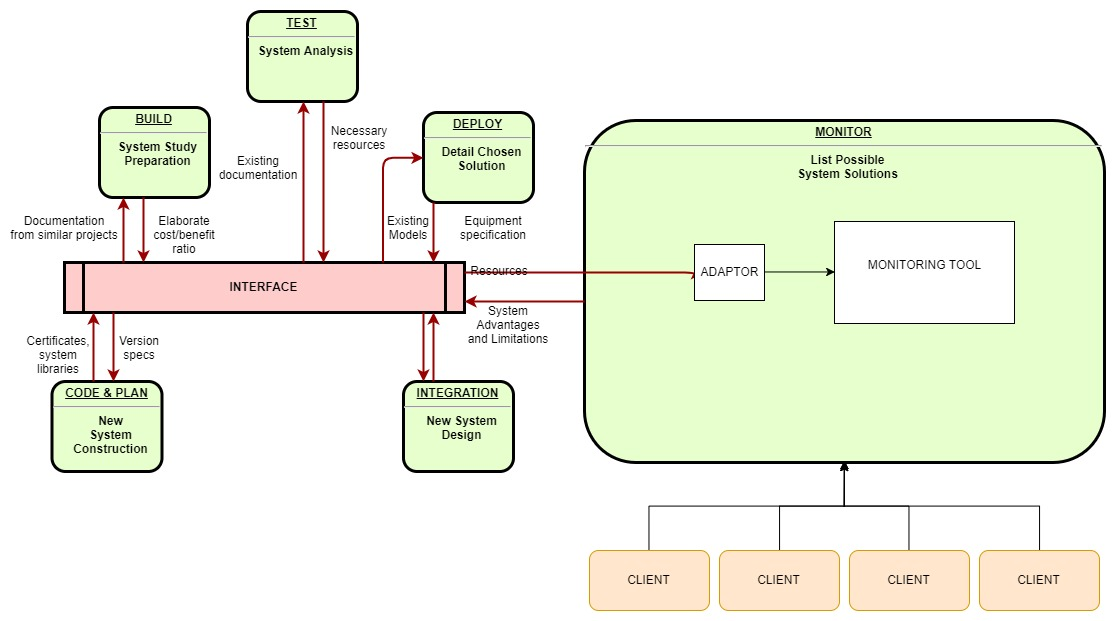
\includegraphics[scale=0.3]{schema.jpg}
\caption{Project Schema \label{overflow}}
\end{figure}



\subsection{References}
     
Zabbix’s website:  
https://www.zabbix.com
\newline
Mule Entreprize Service Bus:
https://www.mulesoft.com
\newline
Zabbix’s github:
https://github.com/zabbix
\newline
IEEE Template for System Requirement Specification Documents:
https://goo.gl/nsUFwy
\newline
Zabbix’s requirements:
https://www.zabbix.com/documentation/3.0/manual/installation/requirements

\section{Overall Description}

    \subsection{Product Perspective}

     This project  is developed for everyone who is interested in developing applications in DevOps logic and wants to monitor them so that he can enhance their performance or just experiment with the feature so that he can understand it and use it as a means of analyzing performance of his/her project.

\subsection{Product Functions}

	GTU CSE343 DevOps Portal Project has seven branches implementing  parts of the DevOps. The  monitoring part using Mule ESB and Zabbix has a simple user interface where Zabbix server can be accessed. It provide a link to the main page of monitoring that shows the programs that are developed in the portal. You can access the following features of the project.
\flushleft
Monitor:

\begin{itemize}
	\item[$\bullet$] 
Create User: This method allows to create new users. Additionally to the standard user properties, the method accepts the following parameters. It requires user's password as a  string and array of user groups to add the user to.  Returns an object containing the IDs of the created users under the userids property. The order of the returned IDs matches the order of the passed users.
	\item[$\bullet$] 
Update User: This method allows to update existing users. It requires user properties to be updated as a parameter. The userid property must be defined for each user, all other properties (user's password, user groups to replace existing user groups, the user groups must have the usrgrpid property defined, medias to replace existing medias) are optional. Only the passed properties will be updated, all others will remain unchanged. It returns an object containing the IDs of the updated users under the userids property. The method returns an object containing the ID of the updated user under the userids property.
	\item[$\bullet$] 
Update Profile User: This method allows to update the currently logged in user.  Parameters are user properties to be updated. The userid property must not be defined. Only the passed properties will be updated, all others will remain unchanged. Additionally to the standard user properties, the method accepts user's password, user groups to replace existing user groups, the user groups must have the usrgrpid property defined.  Returns an object containing the ID of the updated user under the userids property. 

 \item[$\bullet$]Delete User : This method allows to delete users. It requires IDs of users to delete and  returns an object containing the IDs of the deleted users under the userids property. 

\item[$\bullet$]Get User: The method allows to retrieve users according to the given parameters. The method supports the parameters  user ID, user IDs group, media ID, etc. Returns either an array of objects or the count of retrieved objects, if the countOutput parameter has been used.

\item[$\bullet$] Login User: This method allows to log in to the API and generate an authentication token.  It requires as  parameters user name and password.If the userData parameter is used, returns an object containing information about the authenticated user.

\item[$\bullet$] Logout User : This method allows to log out of the API and invalidates the current authentication token. The method accepts as a parameter an empty array. Returns true if the user has been logged out successfully.

\item[$\bullet$]Create Host: Create a host called “Linux server”(or any name you like) with an IP interface, add it to a group, link a template to it and set the MAC addresses in the host inventory and finally returns unique ID.

\item[$\bullet$]Delete Host: This method allows to delete hosts. It require IDs of hosts to delete as parameters  and returns an object containing the IDs of the deleted hosts under the hostids property.

\item[$\bullet$]Get Host: The method allows to retrieve hosts according to the given parameters.  Parameters defining the desired output. Some supported parameters are hosts that belong to the given groups, hosts that have the given applications, hosts that are related to the given discovered services, hosts that have the given graphs, hosts with the given host IDs, hosts that have the given web checks, hosts that use the given interfaces. Returns either an array of objects, the count of retrieved objects, if the countOutput parameter has been used.

\item[$\bullet$]Exists Host: This method checks if at least one host that matches the given filter criteria exists.

\item[$\bullet$]Update Host: This method allows to update existing hosts. Host properties to be updated are taken as parameters. The hostid property must be defined for each host, all other properties are optional. Only the given properties will be updated, all others will remain unchanged. Additionally to the standard host properties, the method accepts host groups to replace the current host groups the host belongs to, host groups must have the groupid property defined, host interfaces to replace the current host interfaces, host inventory properties, user macros to replace the current user macros. The method returns an object containing the IDs of the updated hosts under the hostids property.

\item[$\bullet$]Create Host Group:  This method allows to create new host groups.It requires host groups to create. The method accepts host groups with the standard host group properties and returns an object containing the IDs of the created host groups under the groupids property. The order of the returned IDs matches the order of the passed host groups.

\item[$\bullet$]Delete Host Group: This method allows to delete host groups.  It requires  IDs of the host groups to delete.It returns an object containing the IDs of the deleted host groups under the groupids property. A host group can not be deleted if:
it contains hosts that belong to this group only;
it's marked as internal;
it is used by a host prototype;
it is used in a global script.

\item[$\bullet$]Exists Host Group: This method checks if at least one host group that matches the given filter criteria exists.

\item[$\bullet$]Get Host Group: The method allows to retrieve host groups according to the given parameters.  Parameters defining the desired output which can be graph ID, group IDs are taken as input for the method .The method returns either an array of objects or the count of retrieved objects, if the countOutput parameter has been used.

\item[$\bullet$]Update Host Group:This method allows to update existing hosts groups i.e host group properties to be updated. The groupid property must be defined for each host group, all other properties are optional. Only the given properties will be updated, all others will remain unchanged. Returns an object containing the IDs of the updated host groups under the groupids property.

\item[$\bullet$]Create Graph: This method allows to create new graphs. Parameters are graphs to create. Additionally to the standard graph properties, the method accepts graph items to be created for the graph. The method returns an object containing the IDs of the created graphs under the graphids property. The order of the returned IDs matches the order of the passed graphs.

\item[$\bullet$]Delete Graph: This method allows to delete graphs. Parameters are IDs of the graphs to be deleted.  Returns an object containing the IDs of the deleted graphs under the graphids property.

\item[$\bullet$]Exists Graph: This method checks if at least one graph that matches the given filter criteria exists.

\item[$\bullet$]Update Graph: This method allows to update existing graphs or Graph properties. The graph id property must be defined for each graph, all other properties are optional. Only the passed properties will be updated, all others will remain unchanged. Returns an object containing the IDs of the updated graphs under the graph ids property.

\item[$\bullet$]Create Item: This method allows to create new items. Returns an object containing the IDs of the created items under the itemids property. The order of the returned IDs matches the order of the passed items.

\item[$\bullet$]Delete Item: This method allows to delete items.  It take IDs of the items to delete as  parameters. Returns an object containing the IDs of the deleted items under the item IDs property.

\item[$\bullet$]Get Item: The method allows to retrieve items according to the given parameters. Parameters defining the desired output. Some of parameters supported are item ID, group ID, template ID, graph ID, host ID. The method returns either an array of objects or the count of retrieved objects, if the countOutput parameter has been used.

\item[$\bullet$]Update Item: This method allows to update existing items or item properties.The item ID property must be defined for each item, all other properties are optional. Only the passed properties will be updated, all others will remain unchanged. Returns an object containing the IDs of the updated items under the itemids property.

\end{itemize}

\subsection{User Classes and Characteristics}

\item[$\bullet$]Developers, who wants to monitor the efficiency of the programs they developed.
\item[$\bullet$]Operational users, such as CEO, POs, Scrum Masters, Support Desk, etc. who wants to monitor the clients.

\subsection{Operating Environment}

\item[]On web
\item[]Linux
\item[]Windows 7
\item[]Windows 8
\item[]Windows 10


\subsection{Design and Implementation Constraints}

  The communication between Interface and Monitoring needs an adapter which is developed in Java. The adapter is passed to ESB ( Enterprise Service Bus) which acts as a server to receive and send http request coming from/to monitoring. The DevOps Portal Project monitoring module uses Zabbix Monitoring Tool and Mulesoft API as ESB.


\subsection{User Documentation}

To use this feature to its maximum capacity it requires knowledge of Mule. There is a quick start on how to use mule at 
\newline https://developer.mulesoft.com/tutorials-and-howtos. 

Additional help and information can be found at 343SoftwareEngineering’s wiki:
\newline https://github.com/AhmetOzyilmaz/343SoftwareEngineering/wiki
 
Also Zabbix knowldege is required also. Zabbix official page provides user manuel for starters at https://www.zabbix.com/documentation/3.4/manual

\subsection{Assumptions and Dependencies}
Since the project uses Zabbix to monitor, it requires every requirement that Zabbix needs such as Apache and PHP which can be accessed from the following link to Zabbix requirements page:
https://www.zabbix.com/documentation/3.0/manual/installation/requirements
Adapters that are used to perform communication between the Interface and the monitor modules are developed in Java therefore Java version 7 or higher has to be installed on the computer that will monitor the clients. 
To access the monitoring module as well as the other modules of the DevOps Portal, a web browser with cookies and JavaScript enabled is required as well.

\section{External Interface Requirements}

\subsection{User Interfaces}

In User interface the monitored host are displayed. And for every monitored host the application which it contains that are being monitored can be seen.
\subsection{Hardware Interfaces}
\begin{itemize}
\item[]Memory:
    Zabbix requires both physical and disk memory. 128 MB of physical memory and 256 MB of free disk space could be a good starting point. However, the amount of required disk memory obviously depends on the number of hosts and parameters that are being monitored.
\item[]CPU:
   Zabbix and especially Zabbix database may require significant CPU resources depending on number of monitored parameters and chosen database engine.
\end{itemize}
\subsection{Software Interfaces}

     The project requires Java to be installed on the computer that will monitor. A web browser with cookies and JavaScript enabled is required. The system also needs to provide the requirements for Zabbix. Additional information can be found on section 2.7 of this document.

\subsection{Communications Interfaces}

DevOps Portal Monitoring uses Mule ESB for communication between different parts of the portal. For a new application which is being deployed from deployment part of the portal, a http request is sent to interface through the ESB bus to monitoring. After signal is received and validated if it contains valid information like IP address and the deployed application name to be monitored. Then the information is processed through our end of the ESB bus and signal are sent to zabbix API. from Mule ESB login details of our zabbix server, host information and application information are passed remotely to zabbix. Zabbix handles analysis of host and application in a given host. The same way happens if a undeploy signal is received. Information travels through the Mule ESB bus to monitoring where a host or application is deleted.

\section{System Features}

This section demonstrates monitoring module of GTU CSE343 DevOps Portal Project most prominent features and explains how they can be used.


\subsection{Monitoring All Hosts}

The user  can list all the hosts in DevOps Platform. 

\begin{figure}[H]
\centering
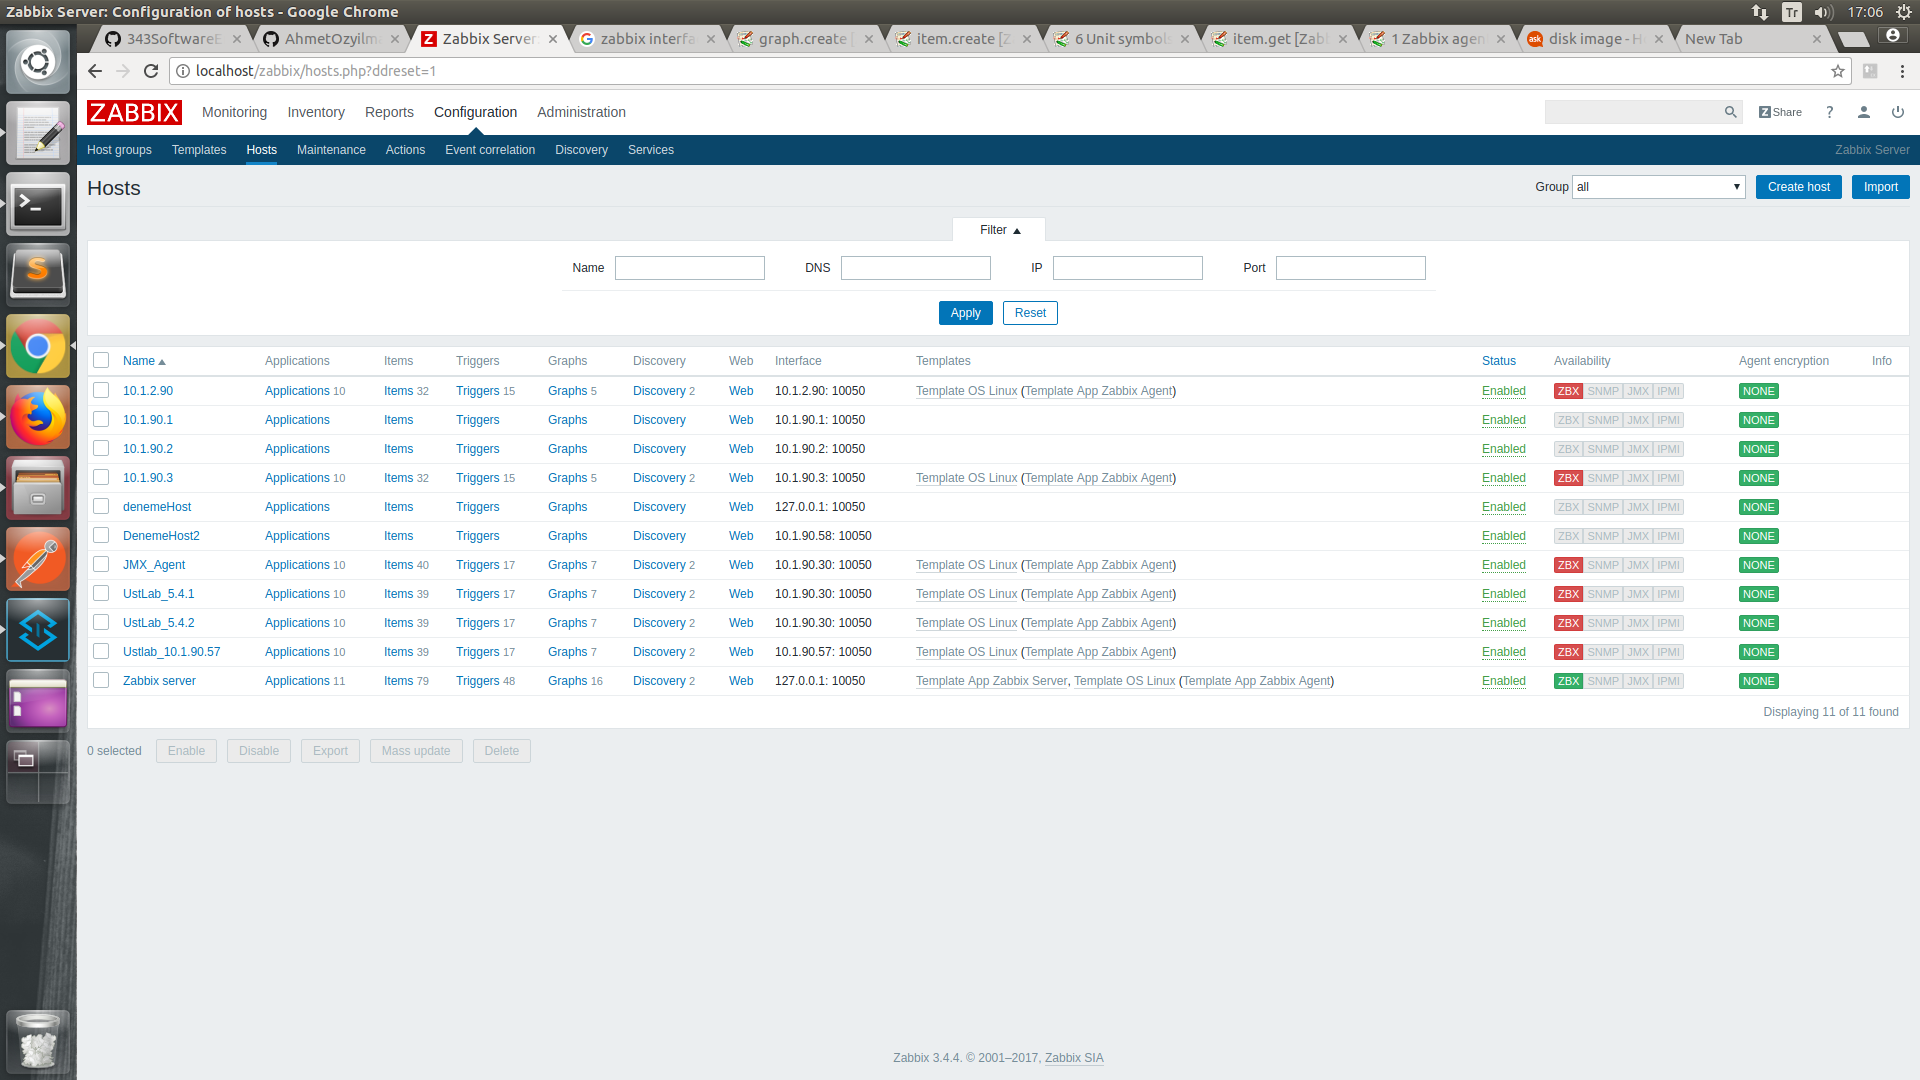
\includegraphics[scale=0.3,width=\linewidth]{ilk_hali01}
\caption{All hosts in the system }
\end{figure}


\subsection{Adding New Host}

The user can add a specific host. The following picture shows that the host which has got 10.1.90.22 ID is created.

\begin{figure}[H]
\centering
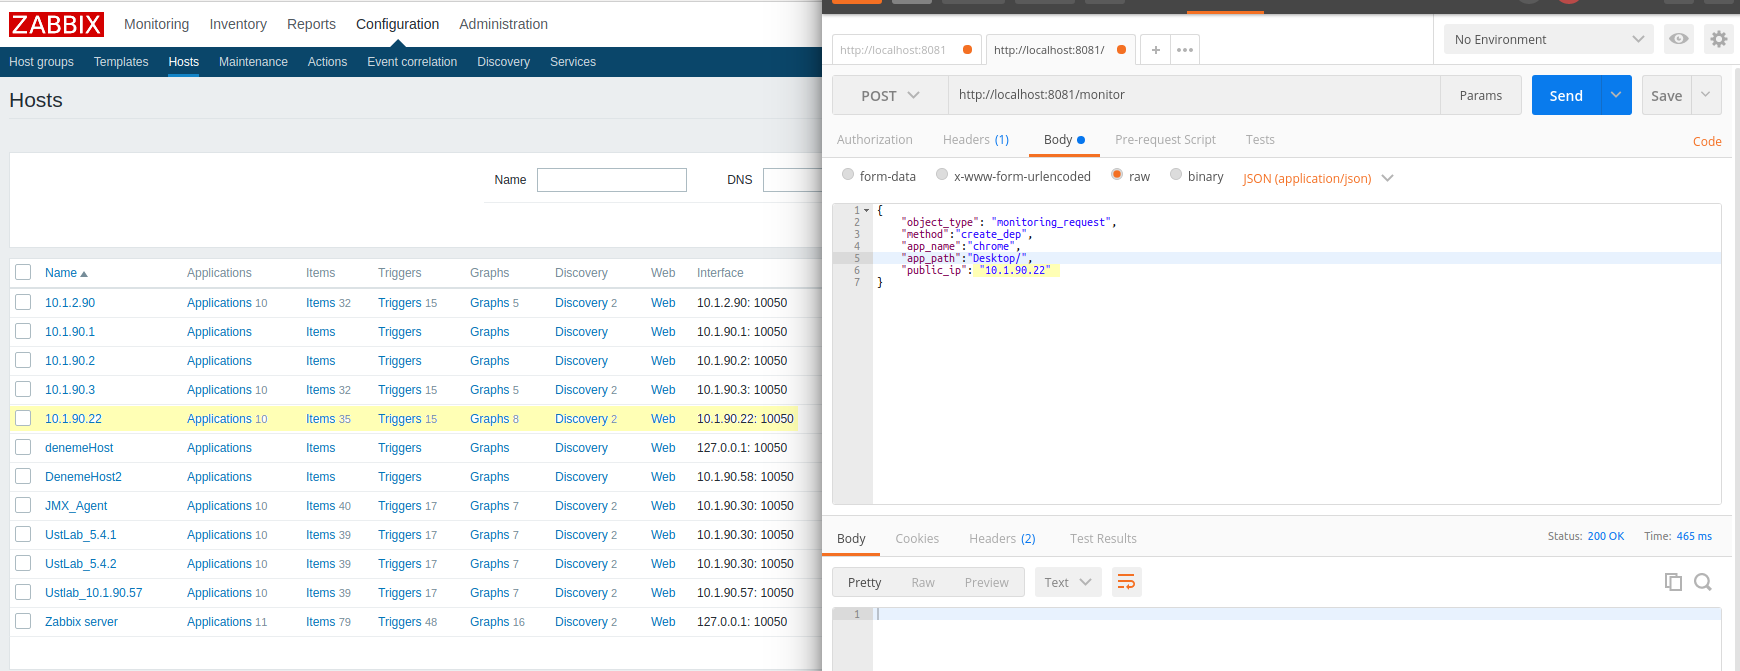
\includegraphics[scale=0.3,width=\linewidth]{eklendi_ilk}
\caption{adding a Host to portal}
\end{figure}



\subsection{ Monitoring Hosts’s Information}

The following picture shows that CPU load information of host which has got 10.1.90.22 ID.

\begin{figure}[H]
\centering
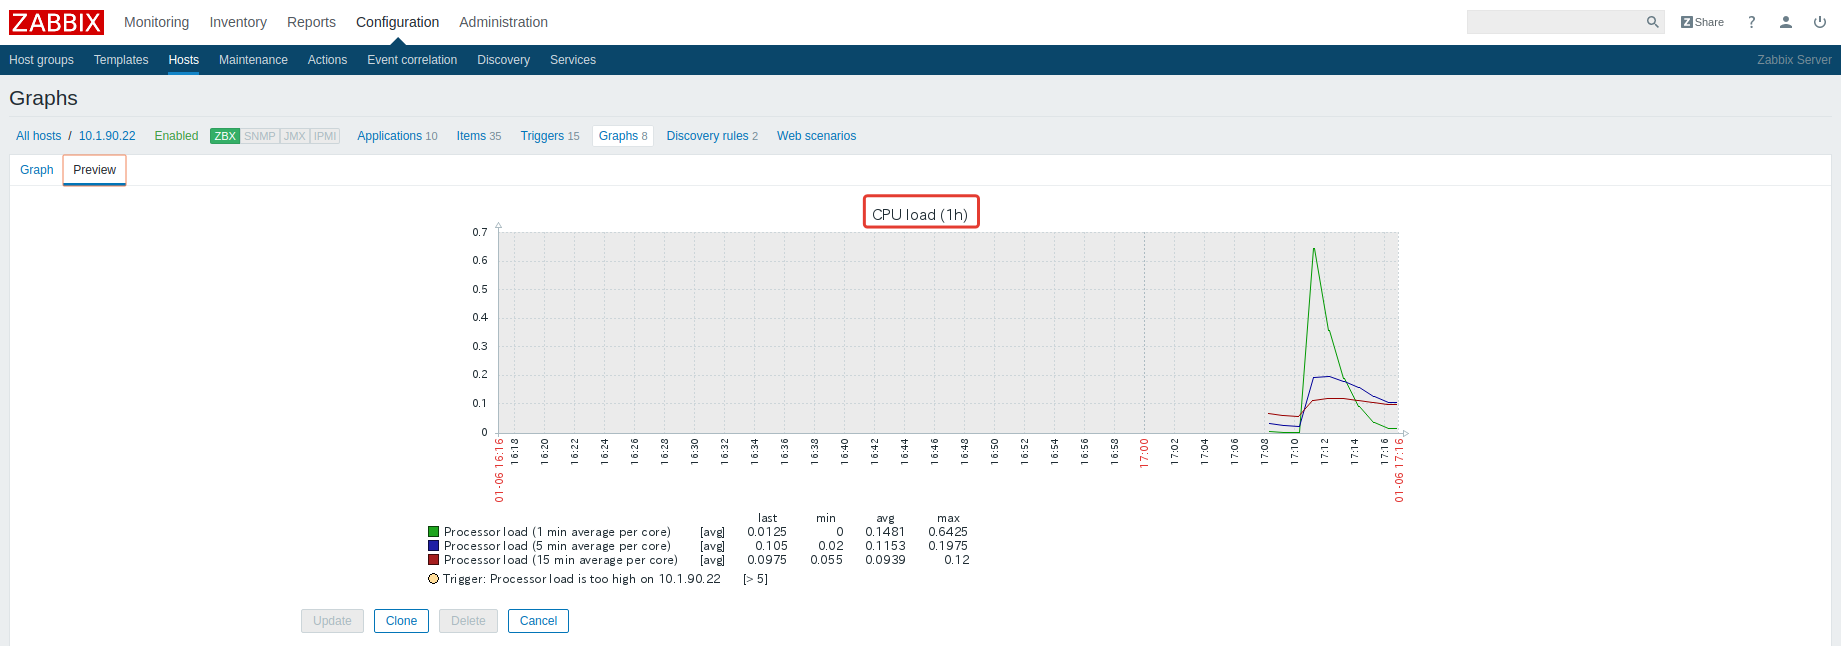
\includegraphics[scale=0.3,width=\linewidth]{ana_host_cpu}
\caption{CPU load Information}
\end{figure}


The following picture shows that memory usage information of host which has got 10.1.90.22 ID.

\begin{figure}[H]
\centering
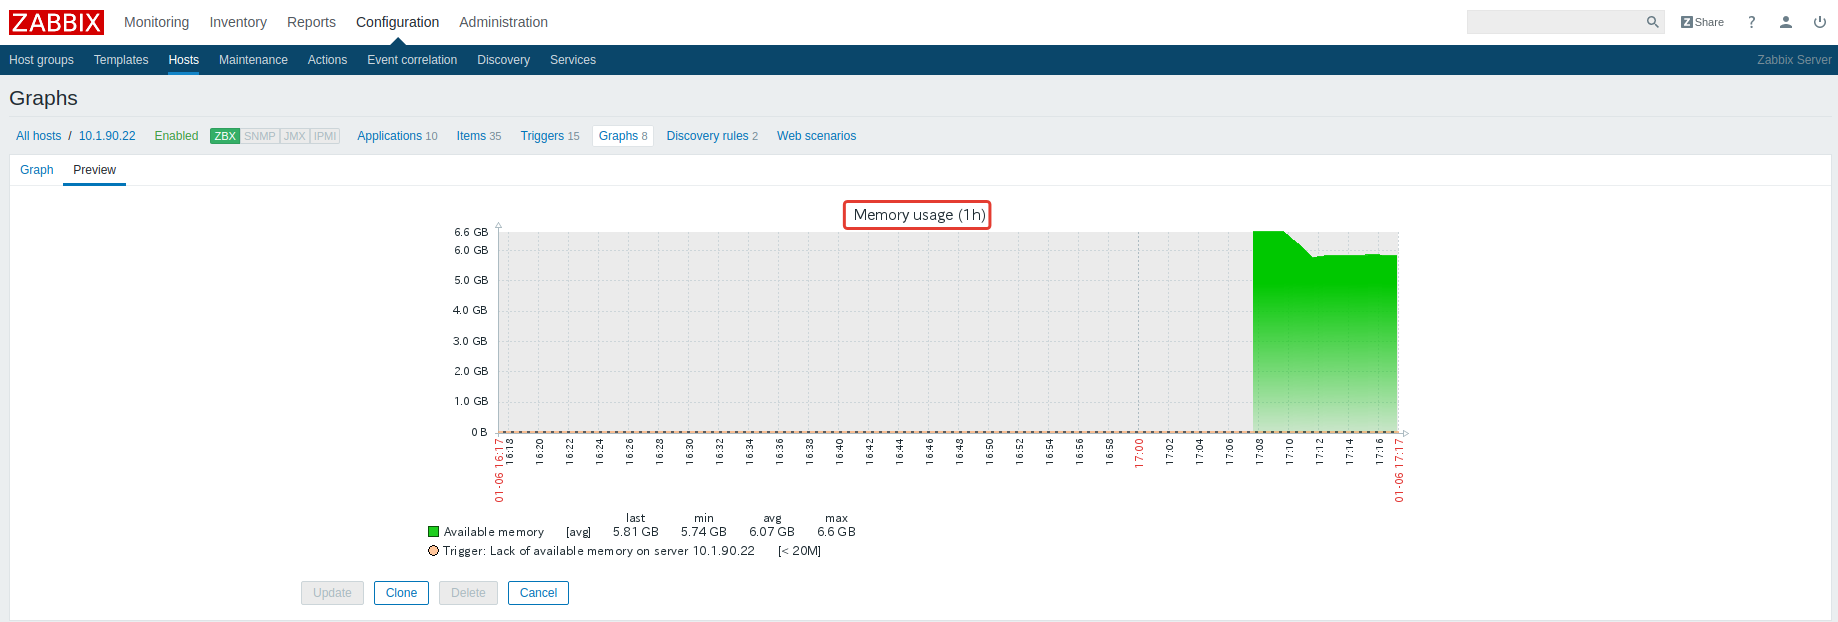
\includegraphics[scale=0.3,width=\linewidth]{ana_host_memory}
\caption{Memory Usage}
\end{figure}



\subsection{ Monitoring Applications in Specific Host}

The following picture shows that the items are created to monitor specific applications in a host. 

\begin{figure}[H]
\centering
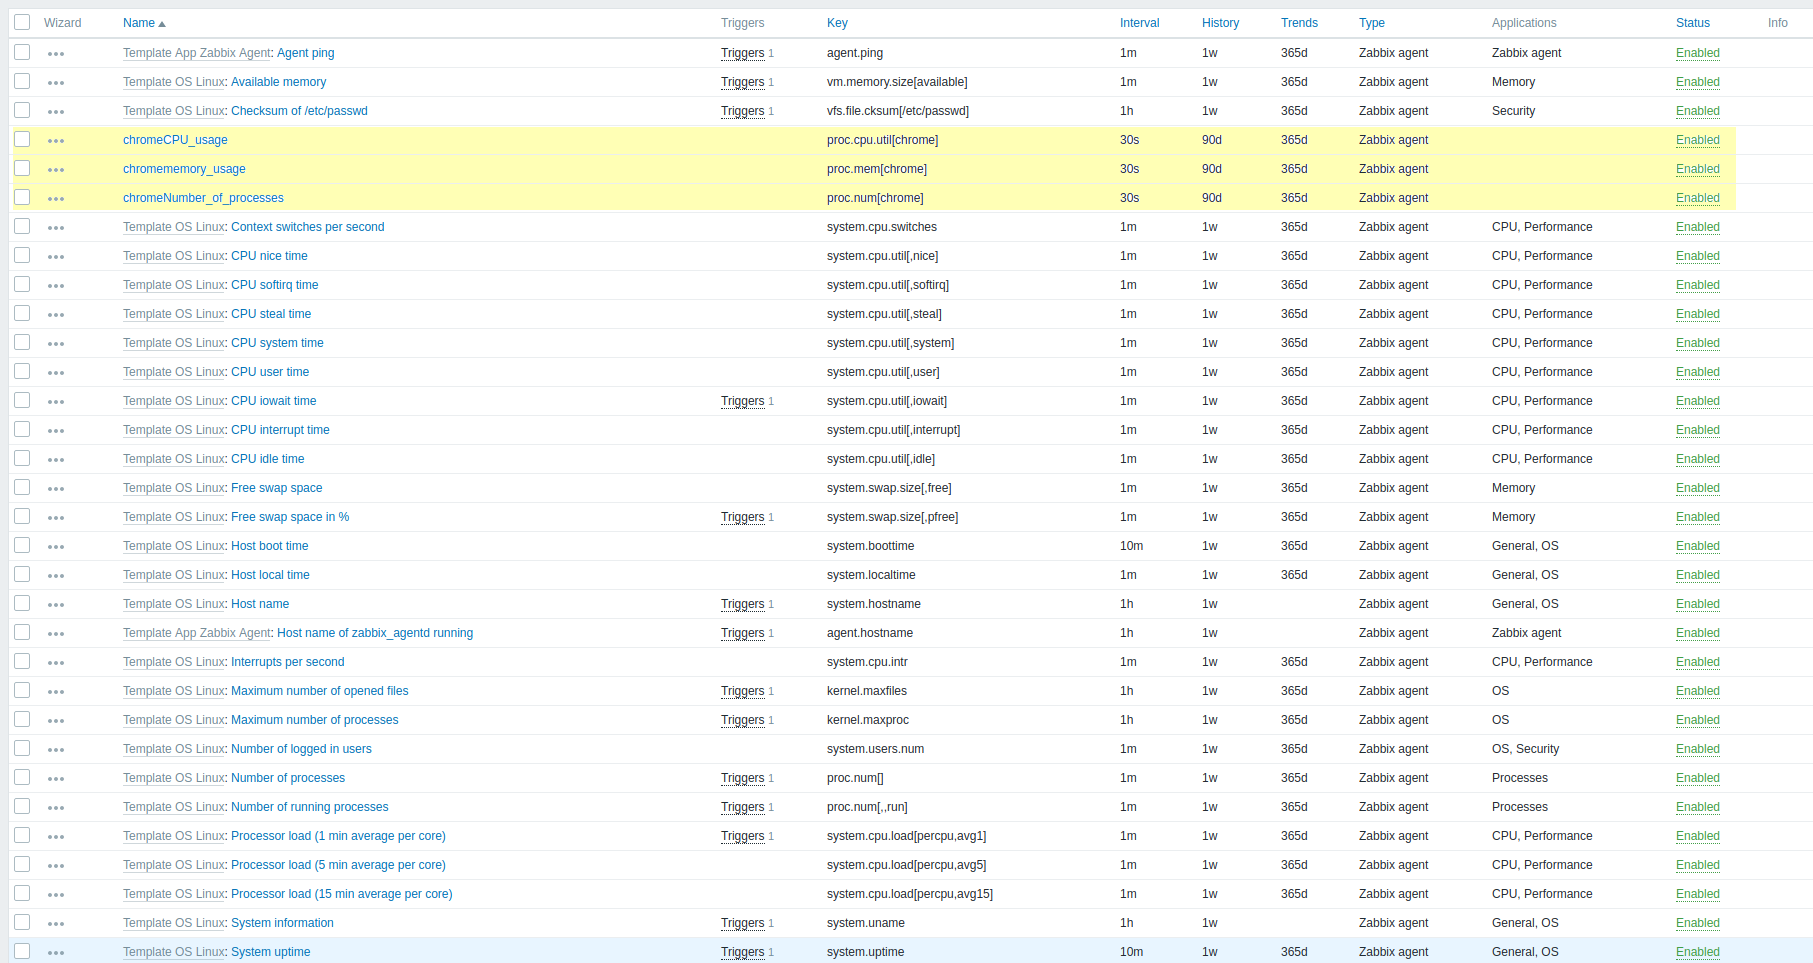
\includegraphics[scale=0.3,width=\linewidth]{item_eklendi1}
\caption{Applications In specific Host}
\end{figure}

A specific application can be monitored and based on its performance necessary modifications can be made.
It shows graphs and how they affect a CPU performance.



\subsection{ Viewing Application’s Data}

The following picture shows how application data is viewed. 

\begin{figure}[H]
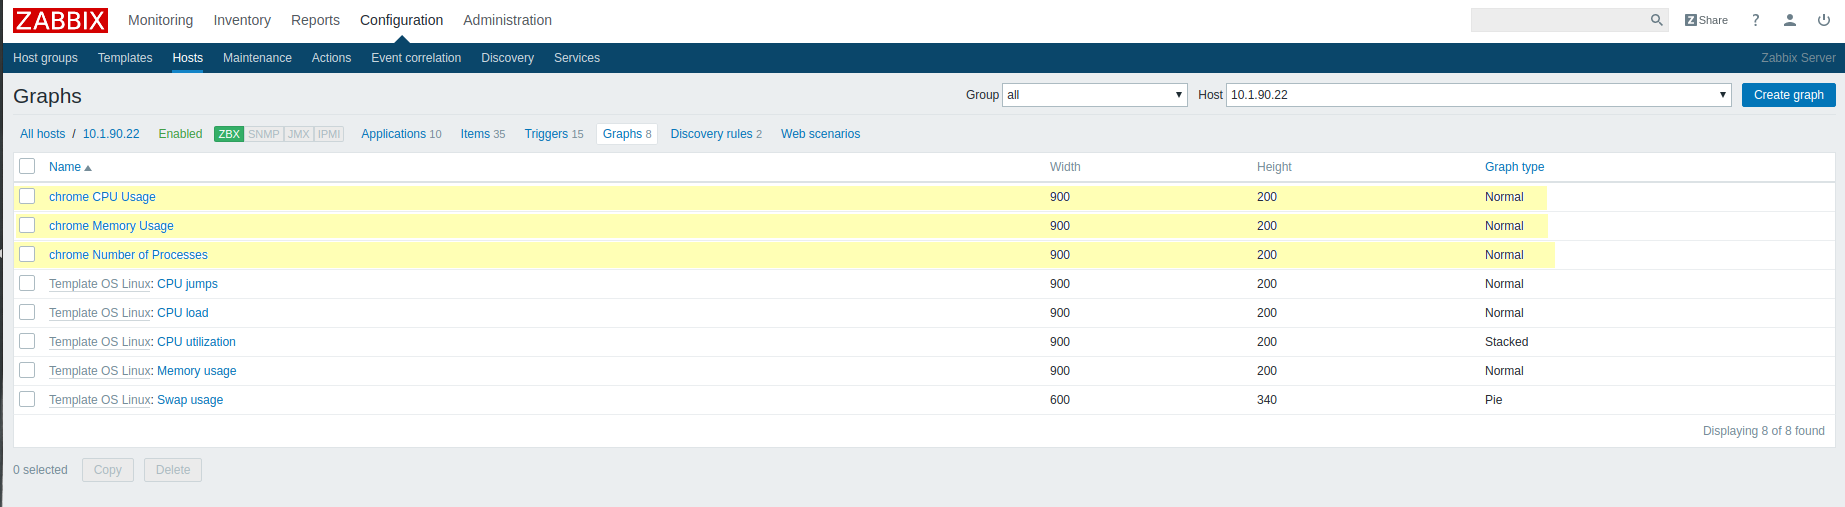
\includegraphics[scale=0.3,width=\linewidth]{graphs_eklendi1}
\caption{Viewing Application's Data}
\end{figure}

\begin{figure}[H]
	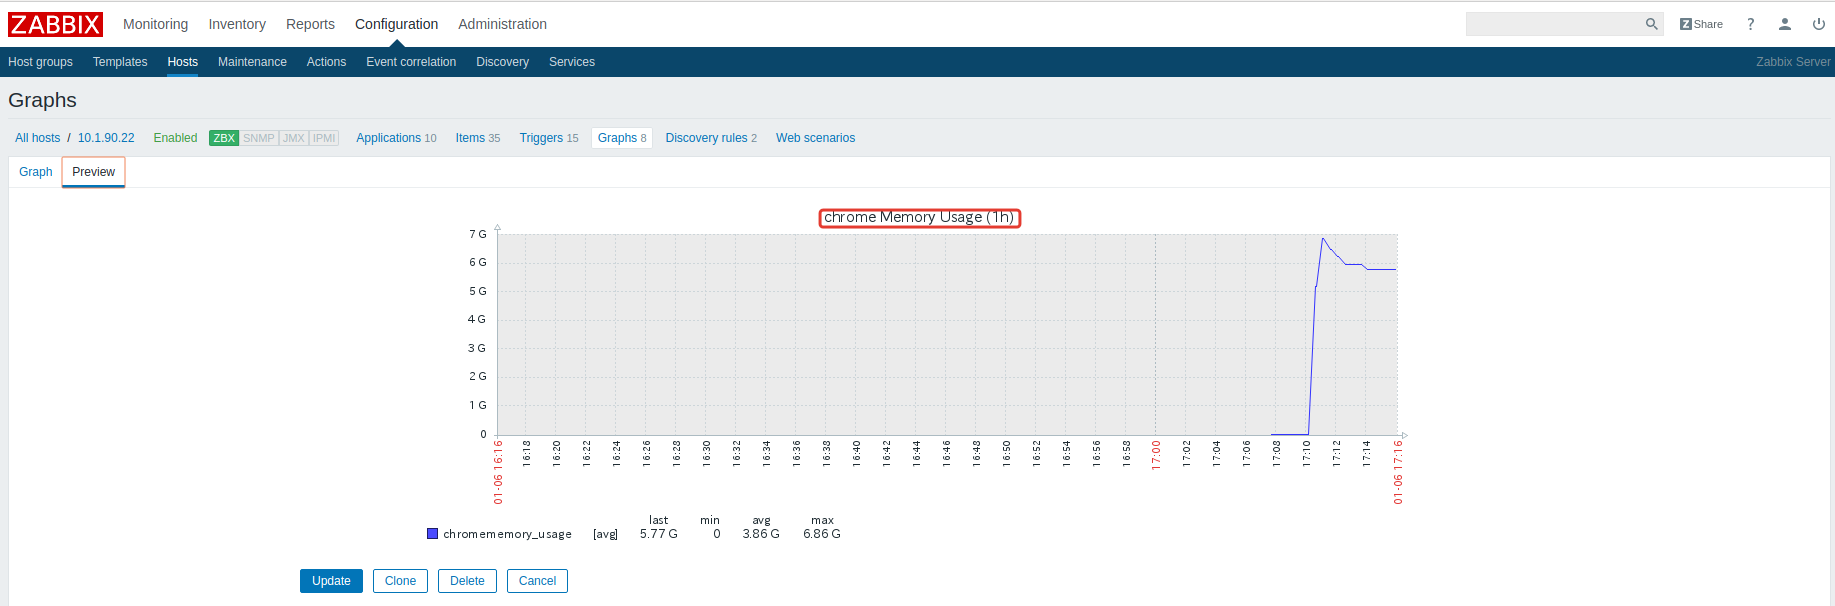
\includegraphics[scale=0.3,width=\linewidth]{memory_usage}
	\caption{Application's Memory Usage}
\end{figure}

\begin{figure}[H]
	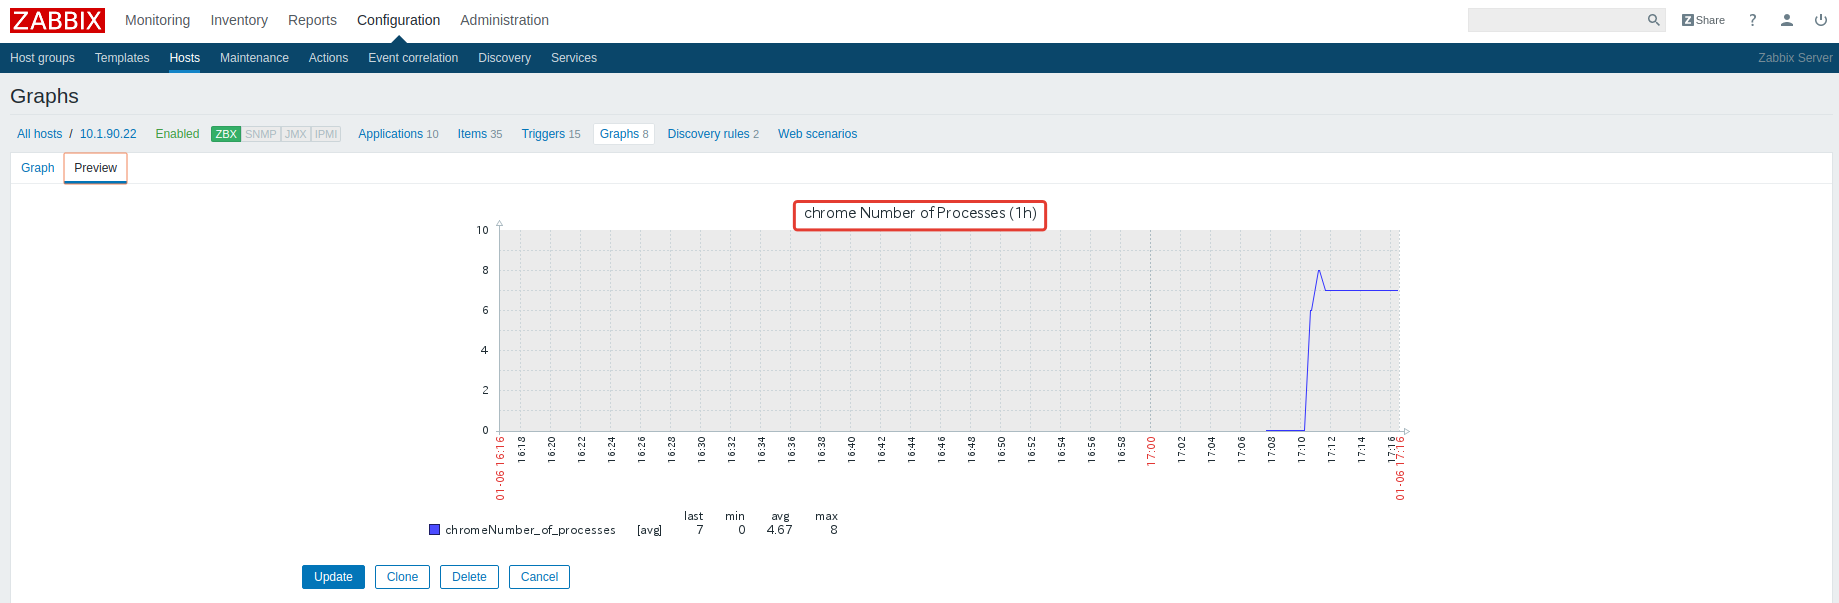
\includegraphics[scale=0.3,width=\linewidth]{number_of_processes}
	\caption{Application's Processes}
\end{figure}

\subsection{Deleting Host}

 When the request to delete host is received through Mule ESB from deploy, a request containing information of a host to be deleted is sent to zabbix server where the host is deleted remotely.





\section{Other Nonfunctional Requirements}

\subsection{Performance Requirements}
\begin{itemize}
\item[]Memory:
    Zabbix requires both physical and disk memory. 128 MB of physical memory and 256 MB of free disk space could be a good starting point. However, the amount of required disk memory obviously depends on the number of hosts and parameters that are being monitored.
\item[]CPU:
   Zabbix and especially Zabbix database may require significant CPU resources depending on number of monitored parameters and chosen database engine.
   
 \end{itemize}
\subsection{Security Requirements}
Zabbix does not have any security requirements and thus any type of user can use it without any additional privileges.

\appendix
\section{Glossary}
\begin{itemize}
\item[$\bullet$]Adapter: In computing, adapter is a hardware or software device that converts transmitted data from one presentation form to another.
\item[$\bullet$] Client: A client is a piece of computer hardware or software that accesses a service made available by a server.
\item[$\bullet$] Cookies: Small files which are stored on a user's computer. They are  designed to hold a modest amount of data specific to a particular client and website, and can be accessed either by the web server or the client computer.
\item[$\bullet$] DevOps: It is a project development philosophy which aims at increasing software         
            productivity by combining development and Operational part of project  together.
\item[$\bullet$]GTU: An acronym for Gebze Technical University.
Server: In computing, a server is a computer program or a device that provides functionality for other programs or devices, called “clients”.
\item[$\bullet$] Web Browser: A web browser is a software application for retrieving, presenting and traversing information resources on the Word Wide Web.
\item[$\bullet$] Zabbix: An open source application monitoring tool.
\end{itemize}


\end{document}
